\documentclass[12pt,a4paper]{article}
\usepackage{amsmath, amssymb}
\usepackage{geometry}
\usepackage{hyperref}
\usepackage{booktabs}
\usepackage{graphicx}
\usepackage{setspace}
\usepackage{float}
\usepackage{tikz}
\usepackage{tikz-uml}
\usepackage{enumitem}

\usetikzlibrary{arrows.meta, positioning}
\usetikzlibrary{shapes.geometric, arrows}


\tikzstyle{terminal} = [rectangle, rounded corners, 
minimum width=3cm, 
minimum height=1cm,
text centered, 
draw=black, 
fill=red!30]

\tikzstyle{io} = [trapezium, 
trapezium stretches=true, % A later addition
trapezium left angle=70, 
trapezium right angle=110, 
minimum width=3cm, 
minimum height=1cm, text centered, 
draw=black, fill=blue!30]

\tikzstyle{process} = [rectangle, 
minimum width=3cm, 
minimum height=1cm, 
text centered, 
% text width=3cm, 
draw=black, 
fill=orange!30]

\tikzstyle{decision} = [diamond, 
minimum width=3cm, 
minimum height=1cm, 
text centered, 
draw=black, 
fill=green!30,
aspect=2.2]
\tikzstyle{arrow} = [thick,->,>=stealth]


\graphicspath{{assets/}}

%title page
\geometry{margin=1in}

\begin{document}

% Title Page
\begin{titlepage}
	\centering
	    
	\Huge
	\textbf{Jaypee Institute of Information Technology, Sector - 62, Noida } \\
	\vspace{0.5cm}
	\Large
	\textbf{B.Tech CSE II Semester}\\
	\vspace{1cm}
	\vspace*{\fill}
	    
	
\includegraphics[scale=0.2]{jiit_logo}\\
	    
	\vspace{1.5cm}
	\Huge
	\textbf{SDF Lab PBL Report}\\
	\Large
	    
	\textbf{Real-Time Chat Application}\\
	\vspace{1cm}
	
	\Large
	\textbf{Submitted to}\\
	Dr. Amarjeet Prajapati \\
	Dr. Anuja Shukla \\
	Dr. Sulabh Tyagi \\
	\vspace{1cm}
	
	\textbf{Submitted by}
	\vspace{0.5cm}
	
	\begin{tabular}{ll}
		Harsh Sharma      & 2401030232 \\
		Karvy Singh       & 2401030234 \\
		Rudra Kumar Singh & 2401030237 \\
	\end{tabular}
	
	\vspace*{\fill}
	\normalsize
\end{titlepage}

%letter of transmittal 
\begin{center}
	\Large\textbf{Letter of Transmittal}
\end{center}
\vspace{1cm}

\noindent
\textbf{Dr. Amarjeet Prajapati} \\
\textbf{Dr. Anuja Shukla} \\
\textbf{Dr. Sulabh Tyagi} \\
[0.5em]
Department of Computer Science \& Information Technology\\
[0.5em]
Jaypee Institute of Information Technology \\
Sector 62, Noida

\vspace{1cm}

\noindent
\textbf{Subject:} Submission of Report on ``Real-Time Chat Application''

\vspace{1cm}

\noindent
Respected Sir,

\vspace{1em}

\noindent
We are pleased to submit our report for our project \textit{``Real-Time Chat Application''} as part of our coursework. This report documents our work throughout the project's lifetime. \vspace{1em}

\noindent
This project is a Real-Time Desktop Chat Application developed in C++ using the Qt framework for the GUI, Boost.Asio for networking, and SQLite for local data storage. It follows an object-oriented approach and supports real-time text messaging, user authentication, and chat history persistence. The system includes a client with a login and chat interface, and a server that handles connections, user management, and message routing. It demonstrates advanced C++ concepts like multithreading, inheritance, virtual functions, and integrates SQL for data handling.
\vspace{1em}

\noindent
We have endeavoured to apply all topics covered in SDF-II and hope that this meets your expectations.
\vspace{1em}

\noindent
Thank you for your guidance and the opportunity to work on this project.

\vspace{2em}

\noindent
Sincerely, \\[2em]

\noindent
Harsh Sharma (2401030232)\\
Karvy Singh (2401030234)\\
Rudra Kumar Singh (2401030237)\\

\vspace{2cm}

\noindent
Date: \today

\newpage

\tableofcontents

\newpage

\section{Introduction}

\subsection{Background and Context}
In the modern era of digital communication, real-time messaging systems have become essential tools for both personal and professional interactions. Traditional communication methods, such as email or SMS, often fail to provide the immediacy and interactivity required in fast-paced environments. As a result, instant messaging platforms have gained widespread popularity for enabling users to exchange messages, files, and multimedia content instantly over a network.

This project stems from the growing need for a \textbf{lightweight, desktop-based chat solution} that prioritizes real-time responsiveness, user-friendly interface design, and secure data management. Built using \textbf{C++} with the \textbf{Qt framework} for GUI and \textbf{Boost.Asio} for networking, the application also incorporates a \textbf{SQLite} database to ensure persistent message storage. This context emphasizes the technical and practical importance of the project in delivering a fully-functional, modular, and extensible communication system.

\subsection{Problem Statement}
Most existing chat applications are either mobile-focused, cloud-dependent, or lack customization for desktop use. Users often have limited control over data, real-time performance is inconsistent, and many tools are not designed for simple local deployment or extensibility. There is a need for a lightweight, desktop-based chat system that provides real-time communication, secure local data handling, and a clean, user-friendly interface—without relying on third-party servers or bloated software stacks.
\subsection{Project Objectives}
The primary objective of this project is to design and implement a desktop-based real-time chat application using C++. The key goals include:

\begin{itemize}

    \item Enable real-time text communication between authenticated users.

    \item Build a responsive and intuitive graphical user interface using Qt.

    \item Implement a secure, local authentication system using SQLite.

    \item Store and retrieve message history efficiently using a local database.

    \item Ensure modular, scalable, and maintainable code using object-oriented principles.

    \item Support future enhancements like profile management, notifications, or group chats.
\end{itemize}
\subsection{Scope of the Project}

This project focuses on building a desktop chat application with core features required for real-time communication. The current scope includes:

\begin{itemize}
    \item User Authentication: Login system with local credential verification using SQLite.

    \item Real-Time Messaging: Instant text message exchange over a custom client-server protocol using Boost.Asio.

    \item Graphical User Interface: Desktop GUI built with Qt for ease of use and interaction.

    \item Message Storage: Local persistence of chat history per user using SQLite.

    \item OOP-Based Architecture: Implementation using object-oriented design for better maintainability and extensibility.

\end{itemize}
The scope does not include mobile support, end-to-end encryption, media file transfer, or cloud-based deployment in this version. However, the system is designed to allow easy integration of these features in future iterations.

  \section{Architecture and Design}

  \subsection{Overview}
  The Real-Time Chat Application is based on a modular, client-server architecture tailored for desktop systems. Implemented in \texttt{C++}, it integrates libraries like \texttt{Qt} for the graphical user interface, \texttt{Boost.Asio} for asynchronous networking, and \texttt{SQLite} for local data persistence. The system design emphasizes object-oriented principles, aiming for scalability, clarity, and extensibility.
  


\subsection{Flowchart}

A flowchart depicting the application's control flow is presented on the following page.
\newpage
% \thispagestyle{empty}
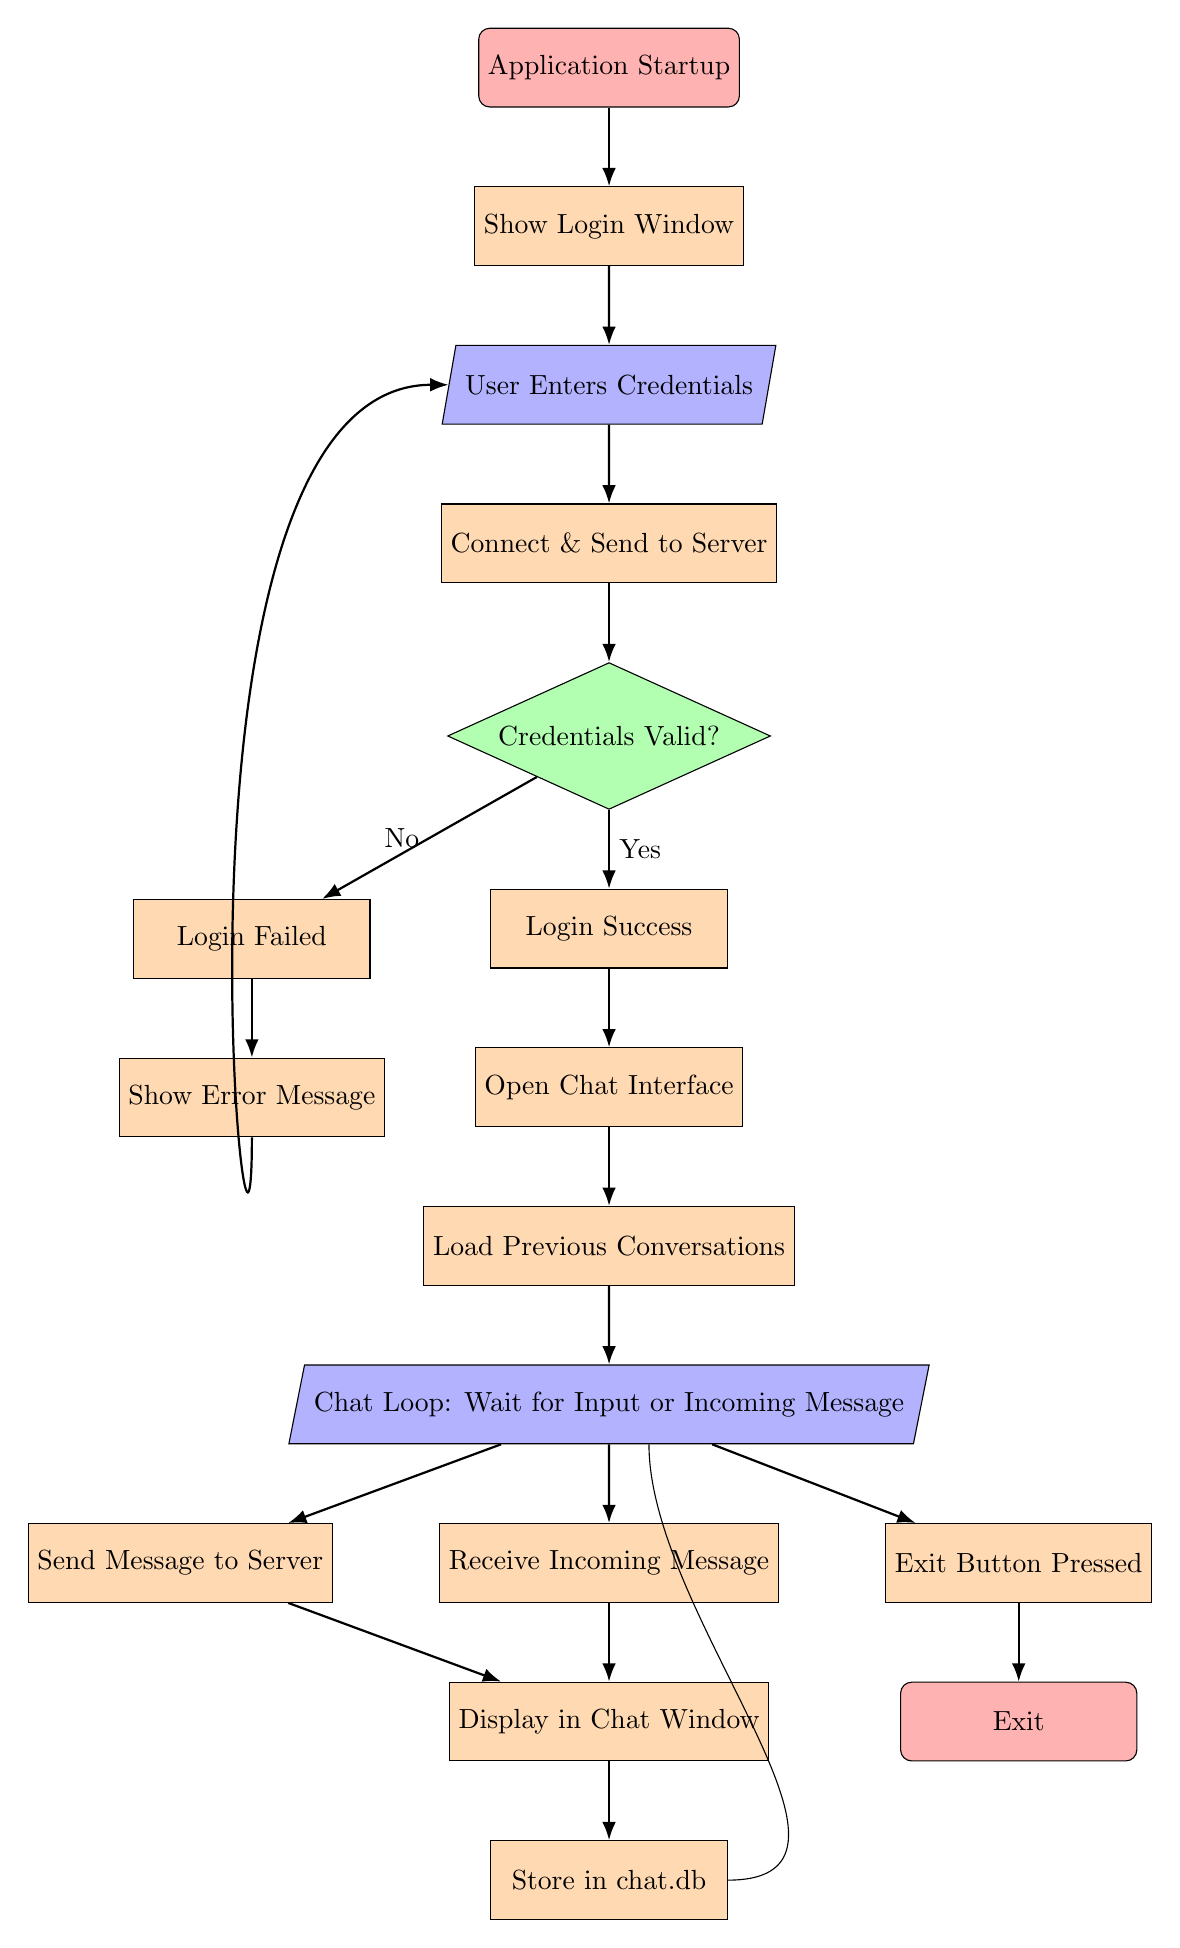
\begin{tikzpicture}[
	% node distance=1cm and 2cm,
	arrow/.style={-{Latex}, thick},
  ]
  
  % Nodes with appropriate flowchart shapes
  \node[terminal] (start) {Application Startup};
  \node[process, below=of start] (loginwin) {Show Login Window};
  \node[io, below=of loginwin] (credentials) {User Enters Credentials};
  \node[process, below=of credentials] (connect) {Connect \& Send to Server};
  \node[decision, below=of connect] (verify) {Credentials Valid?};
  
  \node[process, below left=1.6cm and 2cm of verify] (fail) {Login Failed};
  \node[process, below=of verify] (success) {Login Success};
  \node[process, below=of fail] (error) {Show Error Message};
  
  \node[process, below=of success] (chatui) {Open Chat Interface};
  \node[process, below=of chatui] (loadchat) {Load Previous Conversations};
  \node[io, below=of loadchat] (chatloop) {Chat Loop: Wait for Input or Incoming Message};
  
  \node[process, below left=1cm and 3cm of chatloop] (sendmsg) {Send Message to Server};
  \node[process, below = 1cm of chatloop] (recvmsg) {Receive Incoming Message};
  \node[process, below right=1cm and 3cm of chatloop] (exitmsg) {Exit Button Pressed};
  
  \node[process, below=of recvmsg] (display) {Display in Chat Window};
  \node[process, below=of display] (store) {Store in chat.db};
  \node[terminal, below=of exitmsg] (exit) {Exit};
  
  % Arrows
  \draw[arrow] (start) -- (loginwin);
  \draw[arrow] (loginwin) -- (credentials);
  \draw[arrow] (credentials) -- (connect);
  \draw[arrow] (connect) -- (verify);
  
  \draw[arrow] (verify) -- node[midway, left] {No} (fail);
  \draw[arrow] (verify) -- node[midway, right] {Yes} (success);
  
  \draw[arrow] (fail) -- (error);
  \draw[arrow] (error.south) to[out=-90, in=180] (credentials.west); % Retry loop
  
  \draw[arrow] (success) -- (chatui);
  \draw[arrow] (chatui) -- (loadchat);
  \draw[arrow] (loadchat) -- (chatloop);
  \draw[arrow] (chatloop) -- (sendmsg);
  \draw[arrow] (chatloop) -- (recvmsg);
  \draw[arrow] (sendmsg) -- (display);
  \draw[arrow] (recvmsg) -- (display);
  \draw[arrow] (display) -- (store);
  \draw[arrow] (chatloop) -- (exitmsg);
  \draw[arrow] (exitmsg) -- (exit);
  % Loop back to chat loop
  \draw[loop] (store.east) to[out=0, in=-90] (chatloop.south east);
  
  \end{tikzpicture}
  


  \subsection{System Architecture}
  
  \subsubsection{Client Side}
  The client is a standalone desktop application responsible for user interaction and communication with the server. Key roles of the client include:
  \begin{itemize}
	  \item Managing login and authentication workflows
	  \item Displaying a real-time messaging interface
	  \item Sending and receiving messages asynchronously
	  \item Storing and retrieving chat history from a local SQLite database
  \end{itemize}
  
  \subsubsection{Server Side}
  The server acts as a central hub, managing user sessions and routing messages between clients. It handles:
  \begin{itemize}
	  \item Verifying user credentials through a persistent SQLite database
	  \item Keeping track of active user sessions
	  \item Relaying messages to recipients or notifying senders of delivery issues
  \end{itemize}
  
  \subsection{Component Design}
  
  \begin{itemize}
	  \item \textbf{LoginWindow:} A Qt widget that allows the user to input credentials and connect to the server.
	  \item \textbf{ClientConnection:} Manages TCP socket communication, handles protocol encoding/decoding, and emits signals for UI updates.
	  \item \textbf{ChatWindow:} The main interface for messaging. It supports chat switching, message entry, and real-time display.
	  \item \textbf{Local Database Layer:} Stores chat history and recent contacts using \texttt{SQLite}.
	  \item \textbf{ChatServer:} Accepts client connections, manages sessions, and delegates communication logic.
	  \item \textbf{Connection:} Represents individual client sessions, handles message processing and disconnection logic.
  \end{itemize}
  

\subsection{Class Diagram}
\begin{tikzpicture}

% Client Classes
\umlclass[x=0, y=0]{LoginWindow}{
+ QLineEdit user \\
+ QLineEdit pass
}{
+ doLogin() \\
+ loginGood() \\
+ loginBad()
}

\umlclass[x=5, y=0]{ClientConnection}{
- socket: tcp::socket \\
- username: string
}{
+ connectTo() \\
+ login() \\
+ sendText() \\
+ handlePacket()
}

\umlclass[x=0, y=-5]{ChatWindow}{
- cur: QString \\
- chatItems: QHash \\
- scrollLay: QVBoxLayout*
}{
+ sendMsg() \\
+ gotMsg() \\
+ addChat() \\
+ rebuild()
}

\umlclass[x=5, y=-5]{LocalDB}{
- db: sqlite3*
}{
+ dbInsert() \\
+ dbLoadChat() \\
+ dbRecentPartners()
}

% Server Classes
\umlclass[x=11, y=0]{ChatServer}{
- connections: map \\
- acceptor: tcp::acceptor
}{
+ handleLogin() \\
+ handleChatMessage() \\
+ sendPacket() \\
+ start()
}

\umlclass[x=11, y=-5]{Connection}{
- socket: tcp::socket \\
- username: string
}{
+ start() \\
+ doReadHeader() \\
+ handleMessage() \\
+ send()
}

% Associations
\umlassoc{LoginWindow}{ClientConnection}
\umlassoc{ChatWindow}{ClientConnection}
\umlassoc{ChatWindow}{LocalDB}
\umlassoc{ChatServer}{Connection}
\umlassoc{ClientConnection}{ChatServer}

\end{tikzpicture}
  \subsection{Communication Protocol}
  
  A custom binary protocol ensures fast and structured communication between clients and the server. The format includes:
  \begin{itemize}
	  \item \textbf{4 bytes:} Magic header (``J'', ``I'', ``I'', ``T'')
	  \item \textbf{1 byte:} Packet type (e.g., login = \texttt{0x01}, message = \texttt{0x02})
	  \item \textbf{4 bytes:} Payload length in big-endian format
	  \item \textbf{N bytes:} JSON-encoded message payload
  \end{itemize}
  
  This hybrid format combines binary framing (for performance) and JSON (for flexibility), allowing the protocol to evolve without breaking compatibility.
  
  \subsection{Design Principles and Patterns}
  
  The application follows established object-oriented practices:
  \begin{itemize}
	  \item \textbf{Encapsulation:} Separation of UI, networking, and storage logic into independent modules.
	  \item \textbf{Event-Driven Architecture:} Implemented using Qt's signal-slot mechanism for responsive UIs.
	  \item \textbf{Memory Safety:} Server components use smart pointers (\texttt{std::shared\_ptr}) for lifetime management.
	  \item \textbf{Efficient Data Structures:} STL containers such as \texttt{std::vector}, \texttt{std::map}, and \texttt{QString} simplify internal data handling.
  \end{itemize}
  
  \subsection{Flow Control}
  
  The flow of the application is reactive and asynchronous, designed to keep the interface responsive while continuously managing communication.
  
  On the \textbf{client side}, the application begins by displaying a login window. Upon entering credentials, a connection is made to the server using Boost.Asio. If authentication is successful, control moves to the main chat interface.
  
  At this point, the system enters a continuous loop where it:
  \begin{enumerate}
	  \item Waits for user input to send a message.
	  \item Listens for incoming messages from the server.
	  \item Updates the chat display accordingly and stores the data locally.
  \end{enumerate}
  
  These operations are performed on separate threads: Qt handles the GUI thread, while Boost.Asio operates in the background for network I/O. This ensures that incoming messages can be processed even while the user is typing or interacting with the interface.
  
  On the \textbf{server side}, asynchronous callbacks are used to accept new connections, parse incoming packets, and respond appropriately. Once a client sends a login or message packet, the server handles it based on its type and either forwards it or replies with an appropriate notification.
  
  This flow architecture makes the application highly responsive and capable of handling multiple concurrent users without blocking or UI delays. The separation of concerns between GUI, networking, and storage also makes the system easier to debug, extend, and maintain.
  
\newpage
  \section{Screenshots}

  This section presents screenshots of key components of the application interface, demonstrating its functionality and user experience.
  
  \begin{figure}[H]
      \centering
      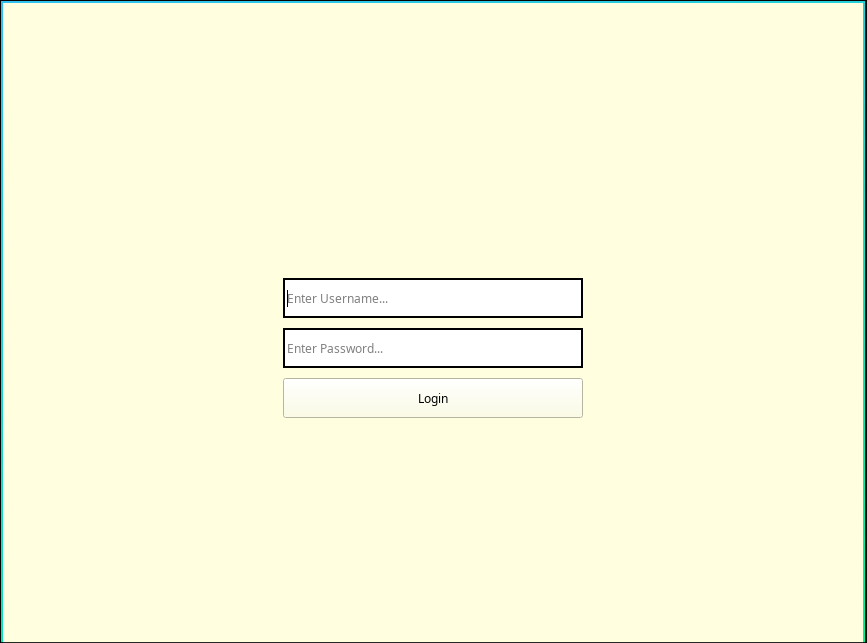
\includegraphics[width=0.75\textwidth]{login.png}
      \caption{Login Window – User enters credentials to connect to the server.}
  \end{figure}
  
  \begin{figure}[H]
      \centering
      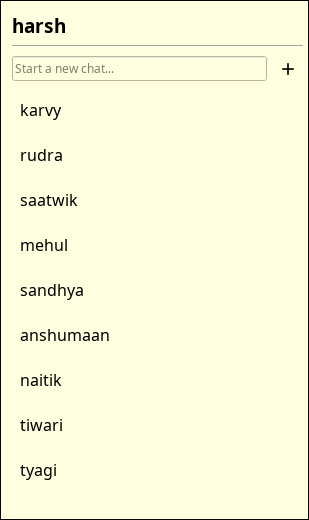
\includegraphics[width=0.4\textwidth]{contacts.png}
      \caption{Contacts – List showing previous conversations.}
  \end{figure}
  \begin{figure}[H]
      \centering
      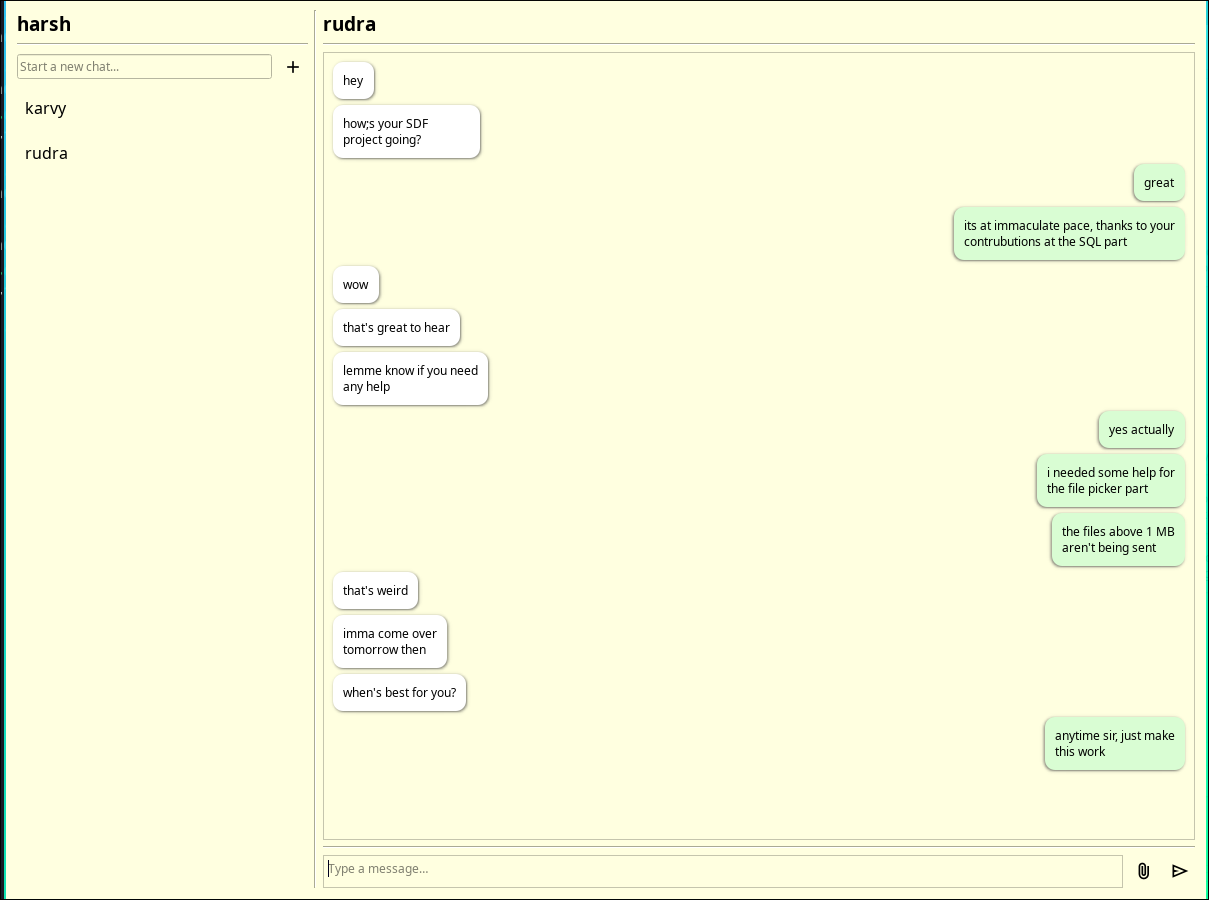
\includegraphics[width=0.75\textwidth]{chat.png}
      \caption{Chat Interface – Real-time messaging window with contacts and message bubbles.}
  \end{figure}
  
  


\section{Conclusion}

\subsection{Summary}
This project successfully demonstrates the design and implementation of a real-time desktop chat application using C++. The application provides core features such as user authentication, real-time text messaging, persistent local storage of chat history, and a clean graphical interface.

By employing modern C++ libraries like \href{https://doc.qt.io/}{Qt} for GUI design and \href{https://www.boost.org/doc/libs/release/doc/html/boost_asio.html}{Boost.Asio} for asynchronous networking, along with a lightweight \href{https://www.sqlite.org/index.html}{SQLite} backend, the system maintains modularity, efficiency, and responsiveness. The project also reinforces object-oriented principles and multi-threaded event handling in a practical context.

\subsection{Future Work and Recommendations}
While the current version meets the core requirements of a real-time desktop chat application, several enhancements are envisioned to improve functionality and user experience:

\begin{itemize}[leftmargin=1.5em]
  \item \textbf{End-to-End Encryption:} Implementing secure encryption to protect message contents during transmission.
  \item \textbf{Group Chat Functionality:} Enabling users to create and participate in multi-user chat groups.
  \item \textbf{Forward Messages:} Allowing users to forward previously received messages to other users or groups.
  \item \textbf{Typing Indicators:} Showing real-time feedback when a user is composing a message.
  \item \textbf{Voice Messages:} Supporting the recording and sending of short audio clips.
  \item \textbf{Voice and Video Calling:} Adding real-time audio and video communication between users.
  \item \textbf{Status Messages:} Enabling users to set custom status messages visible to others (e.g., busy, available).
  \item \textbf{Block Feature:} Allowing users to block specific contacts from messaging or viewing their status.
\end{itemize}


Continued refinement of the codebase, proper unit testing, and integration of deployment tools would also contribute to making the application production-ready.

\section{References}

\begin{enumerate}[label={[R\arabic*]}]
  \item \href{https://www.qt.io}{Qt Framework Documentation} – \url{https://www.qt.io}
  \item \href{https://www.boost.org/doc/libs/release/doc/html/boost_asio.html}{Boost.Asio Networking Library} – \url{https://www.boost.org/doc/libs/release/doc/html/boost_asio.html}
  \item \href{https://www.sqlite.org/index.html}{SQLite Database Engine} – \url{https://www.sqlite.org/index.html}
  \item \href{https://en.cppreference.com/w/}{C++ STL Reference (cppreference)} – \url{https://en.cppreference.com/w/}
  \item \href{https://nlohmann.github.io/json/}{nlohmann/json (Modern C++ JSON)} – \url{https://nlohmann.github.io/json/}
  \item \href{https://doc.qt.io/qt-6/signalsandslots.html}{Qt Signals and Slots Documentation} – \url{https://doc.qt.io/qt-6/signalsandslots.html}
\end{enumerate}

\end{document}
